\section{Experiment 3: Visual search in more detail}

\subsection{Methodology}

\paragraph{Stimuli}

A 10,000-frame corpus of consecutive fire images was used.



\paragraph{Subjects}

11 subjects were recruited using a mailing list operated by University College London. All reported normal or corrected-to-normal vision.

\paragraph{Trial structure}

Yes-no delayed match-to-sample with altered sample.
In each trial, a sample was presented first, followed by a single test. Subjects indicated whether they thought the sample corresponded to the test (up arrow) or now (down arrow).

Samples were all one second (50 frames).

Test clips consisted of the sample, surrounded by a pre-clip and a post-clip, which could both be of length zero.



\paragraph{Factors}

The lengths of the pre-clip and the post-clip (which we term prelength and postlength) were picked from (0, 25,50,100) frames or (0, 0.5,1,2) seconds. Each factor thus had four levels, leading to 16 conditions.

\paragraph{Block structure}

We used 30 training trials with both samples and tests of length one second, and no pre-or post-clips.

The experiment was divided into 10 blocks; subjects took a break between each block. There were 40 trials per block (400 trials total). There were 16 conditions (4*4 factors) and 25 trials per condition.


\begin{figure}[H]
\centering
\renewcommand{\arraystretch}{1.8}

      \begin{subfigure}[b]{\textwidth}
\begin{tabular}{ >{\bfseries}r | p{8cm}   }
& \textbf{Experiment 3}\\
\hline
  
Design & 2AFC delayed match-to-sample, with filtered or inverted sample\\                   
Stimuli & 10000-frame corpus\newline
		1 second sample (50 frames)\newline
		variable-length test\\
Factors & prelength:\newline
		(0, 25,50,100) frames or (0, 0.5,1,2) seconds\newline
		postlength:\newline
		(0, 25,50,100) frames or (0, 0.5,1,2) seconds\newline\\

Block design & prelength and postlength varied within blocks\newline
		10 identical blocks\newline
25 trials per condition \newline
40 trials per block \newline
400 trials \\
Training &30 training trials \\
Subjects&11\\
\end{tabular}
\caption{Design summary.}
   \end{subfigure}

\begin{subfigure}[b]{\textwidth}
\centering
                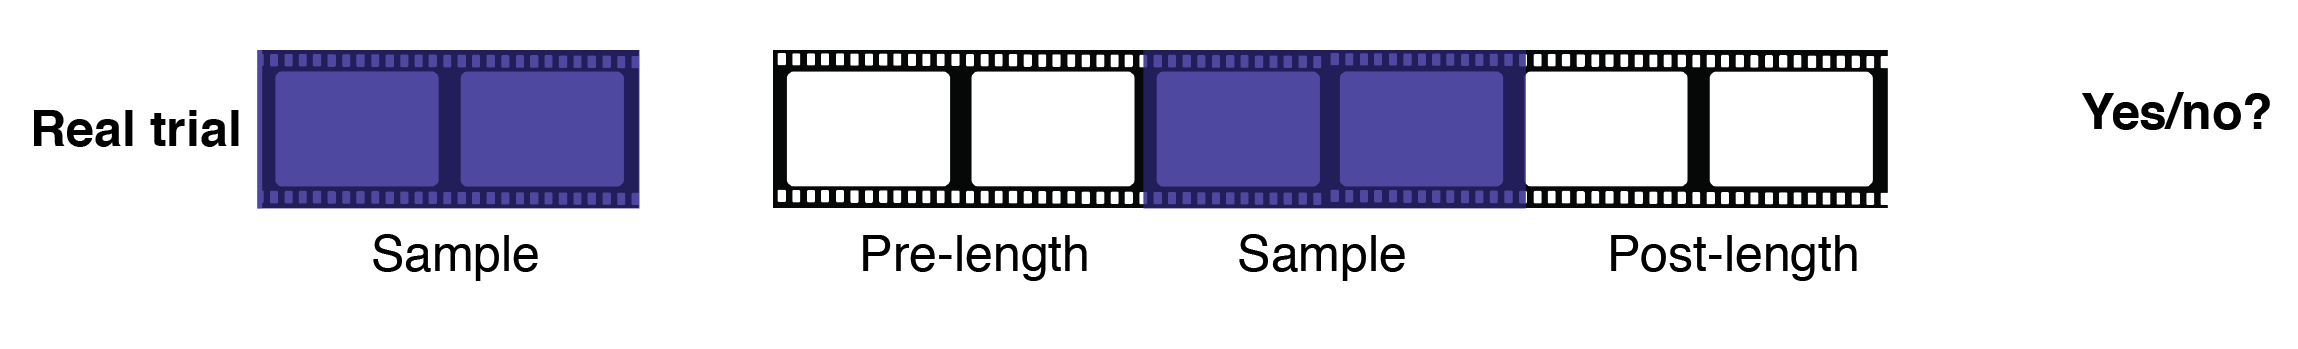
\includegraphics[width=12cm]{img/protocolfire18.png}
                \caption{An altered (filtered or inverted) sample was followed by two untouched tests, one of which contained the sample.}     
        \end{subfigure}
\caption{Experiment 3: design summary and trial structure.}
\end{figure}

\subsection{Results}

\paragraph{Prelength and postlength}

Prelength and postlength could only be defined for the true trials (tests in which the subject was present), not for the foil trials (tests in which the subject was absent).

Over the true trials, a two-way repeated-measures ANOVA revealed no significant effect of prelength or postlength.

\paragraph{Total distractor time and test presence}

The pattern of accuracy in function of total time was related to whether the test was present (true trials) or absent (foil trials). For true trials, accuracy first decreased and then increased as distractor length went up. For foil trials, accuracy smoothly decreased as distractor length went up.

In other words, as distractor length increased:
\begin{itemise}
\item Hits stayed high (with a slight down then up trend), and misses stayed low (with a slight up then down trend)
\item Correct rejects declined, and false positives increased
\end{itemise}

As search space increased, the source of errors is mainly due to false positives, not misses. Accurate judgements were mainly due to hits, not correct rejects. Observers were good at finding a present target, but tended to confuse an absent target for a present one.



\paragraph{Beginning trials and end trials}

We define beginning trials as true trials where the sample was present at the beginning of the test, and end trials as those where the sample was present at the end of the test. In the set of beginning trials, the trial counts by level of postlength were constant; similarly, in the set of end trials, the trial counts by level of prelength were constant. This provided a useful contrast to the analysis by totaltime, where there were neccesarily vastly different numbers of trials at each level.


\paragraph{Signal detection analysis}

As this was a yes/no experiment, we analysed the accuracy pattern using the framework of signal detection theory\cite{green1966signal}. 

First we calculated the collective $d'$ across all subjects for each level of total distractor time. The $d'$ curve followed the same shape as subject accuracy: first descending, then increasing as total time increased.

\paragraph{ROC analysis}

We plotted each subject in ROC space, the 2-$D$ space defined by hit rate over false positive rate\cite{flach2003geometry}.



\begin{figure}[htp]
\centering
\begin{subfigure}[b]{\textwidth}
\centering
                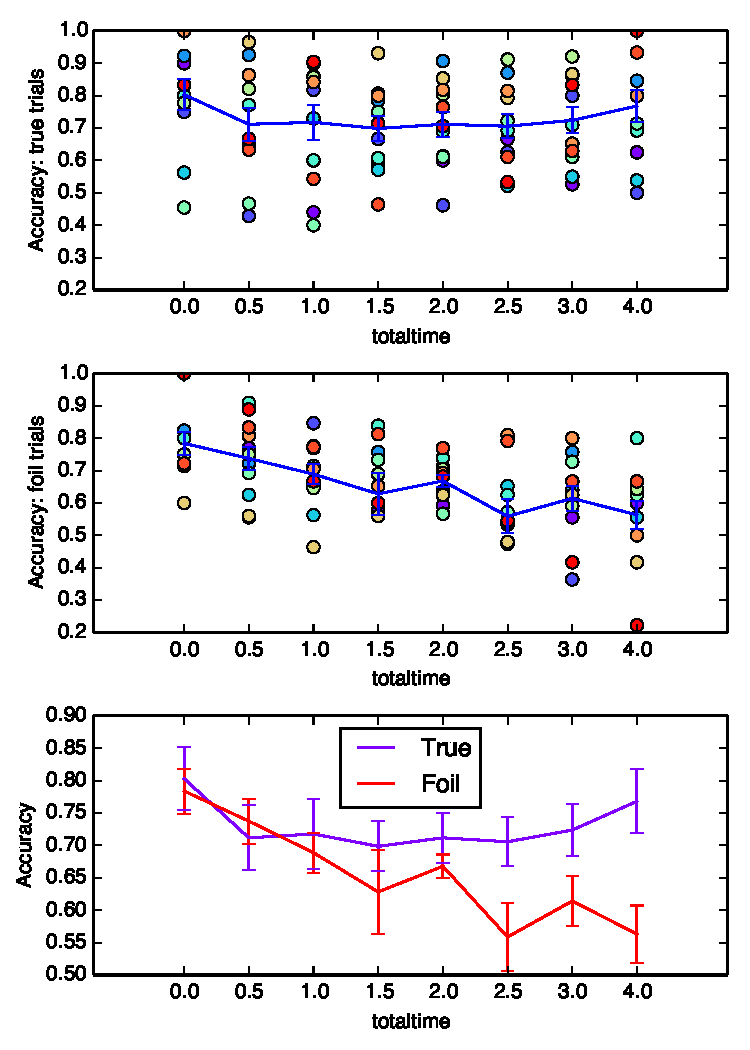
\includegraphics[width=12cm]{img/fig_fire18_totaltime_YN.pdf}
                \caption{Accuracy in function of the five manipulations.}
          
        \end{subfigure}


\caption{Experiment 3: Detection was above chance under all manipulations, but was too low to discern a contrast between the effects.}
\end{figure}

\subsection{Discussion}



Observers were good at finding a present target, but tended to confuse an absent target for a present one. This allows us to rule out a range of search systems: those where the choice of representation was independent of the features observed during the test.
